\documentclass[11pt, a4paper,twocolumn]{jarticle}
\usepackage[dvipdfmx]{graphicx}

\begin{document}
%=============================================================
\section{Signal processing in frequency space (Highpass and lowpass filter) ($5-6^{th} day$)}
% ===============================================================
\subsection{Purpose}
今回の実験では取り込んだ音声信号の周波数空間(フーリエ空間)での信号処理を学ぶ.特定の周波数のみを通す簡単な周波数フィルターの実戦から,窓関数を用いたローパスフィルターおよびハイパスフィルターを学ぶ.
具体的には,異なる共鳴周波数を有する複数の音叉からの音声信号の中から,信号処理によって特定の周波数のみを取り出す.また人が発する高い声と低い声を同時に録音し,信号所によって高い声のみ,または低い声のみを取り出す.
% =======================================================
\subsection{Procedure}
\noindent
\textbf{Task 5.1 特定周波数の取り込み} \\
異なる周波数を有する音叉を二つ選びそれらを同時に鳴らし,音声信号を取得する.
その音声信号を一方のみを通す周波数フィルターをOctaveで政策しフーリエ変換した周波数領域の信号に掛け算する.
次にをれを逆フーリエ変換を行なってスピーカーで鳴らすことで正しく分離できたかを確認するとともにオシロスコープで波の振動数を計測する.
今回は330Hzと440Hzの音叉を同時に鳴らしてフィルターにより440Hzの音叉成分のみを取り出すようなフィルターを用意した.
また今回のサンプリング周波数は20kHz,サンプリング数は20000点とした.

\noindent
\textbf{Task 5.2 ハイパスフィルター,ローパスフィルター} \\
同時に高い声と低い声で異なる言葉を発生し,その声をコンピュータに取り込む.
取り込んだ音声信号をフーリエ変換する.
その後Octaveで窓関数を作り[0,F]までのデータ点数を0,[F+1,40000]までを1にするステップ関数をかけて逆フーリエ変換して低い声がカットされるような整数Fを探した.
今回はサンプリング周波数20kHz,サンプリング数40000点として測定した.
\noindent
\textbf{Task 5.3 ボイスチェンジャー} \\
声を取り込み,周波数を変化させることで,声の高さを変えてスピーカーで再生する.
% =======================================================
\subsection{Result}
\noindent
\textbf{Task 5.1 特定周波数の取り込み} \\
取り込んだ時間領域の声の信号は図\ref{fig:mix}のようになった.
また図\ref{fig:28}はそのうち最初の1000点のみを表示した.
またこの信号のフーリエ変換は図\ref{fig:fftmix}のようになった.
さらにこのフィルター後の関数を逆フーリエ変換したのちスピーカーで再生した.
さらにオシロスコープで周波数を確認すると440Hzの値を得た.

\begin{figure}[htbp]
 \begin{center}
  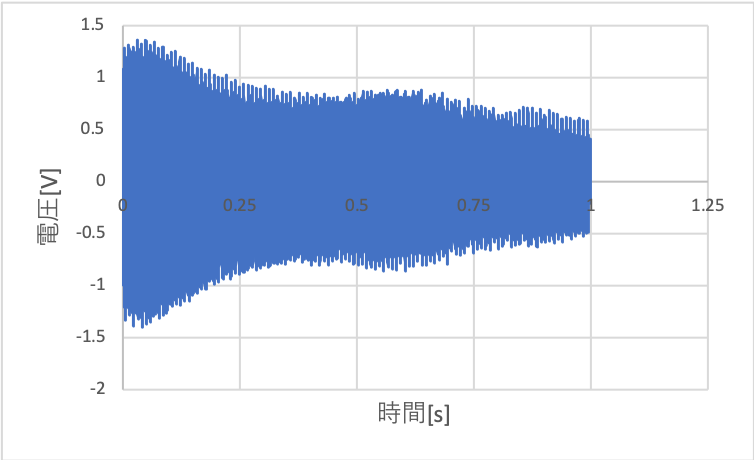
\includegraphics[width=0.8\linewidth]{mix.png}
 \end{center}
 \caption{330Hz,440Hz音叉}
 \label{fig:mix}
\end{figure}

\begin{figure}[htbp]
 \begin{center}
  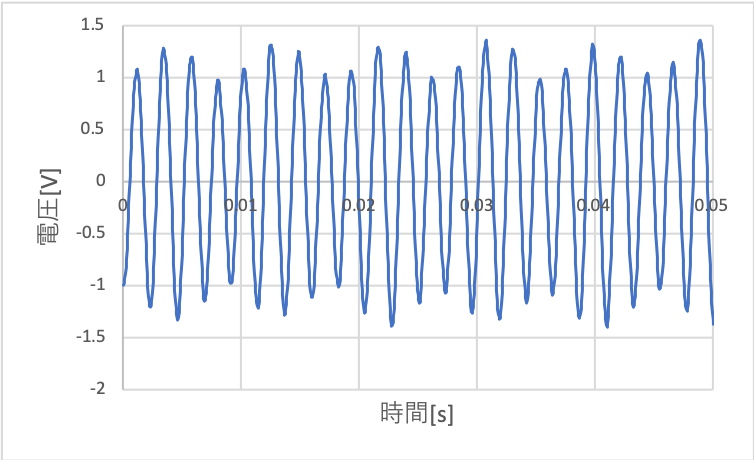
\includegraphics[width=0.8\linewidth]{fig28.png}
 \end{center}
 \caption{330Hz,440Hz音叉}
 \label{fig:28}
\end{figure}

\begin{figure}[htbp]
 \begin{center}
  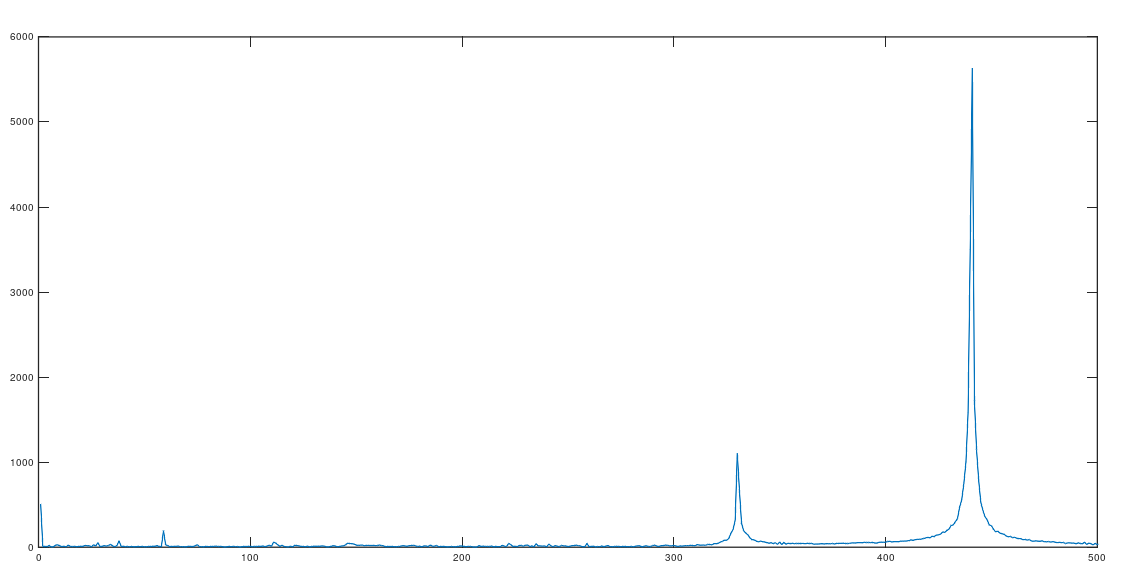
\includegraphics[width=0.8\linewidth]{fftmix.png}
 \end{center}
 \caption{信号のFFT}
 \label{fig:fftmix}
\end{figure}

\begin{figure}[htbp]
 \begin{center}
  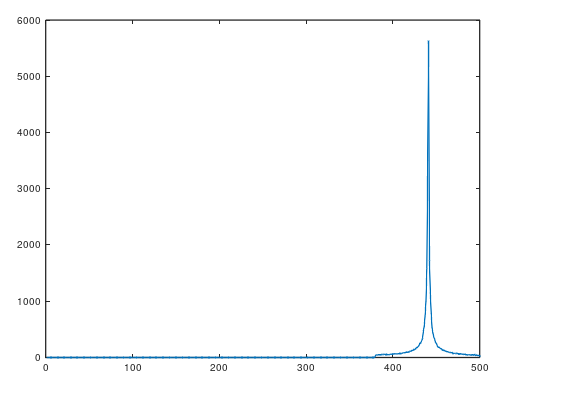
\includegraphics[width=0.8\linewidth]{cfftmix.png}
 \end{center}
 \caption{フィルター後の関数}
 \label{fig:cfftmix}
\end{figure}

\noindent
\textbf{Task 5.2 ハイパスフィルター,ローパスフィルター} \\
取り込んだ音声は図\ref{fig:29}のようになった.
またF = 3000の時低い声がなくなり高い声のみがスピーカーで再生されるようになった.


\begin{figure}[htbp]
 \begin{center}
  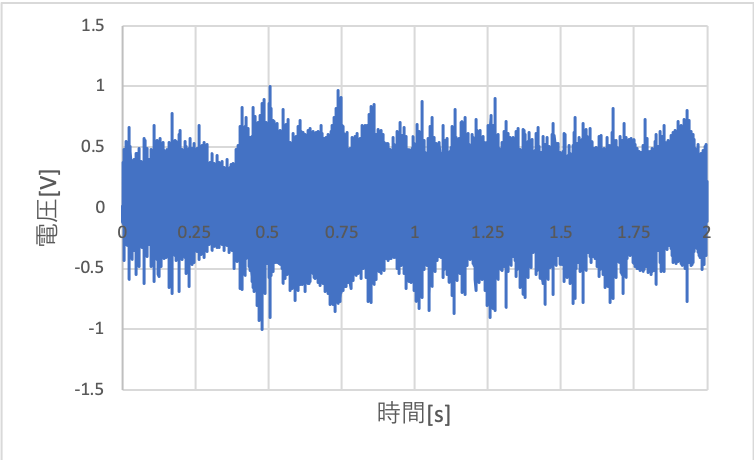
\includegraphics[width=0.8\linewidth]{fig29.png}
 \end{center}
 \caption{取り込んだ声}
 \label{fig:29}
\end{figure}


\noindent
\textbf{Task 5.3 ボイスチェンジャー} \\
前回の実験同様サンプリング周波数をあげて先ほど取り込んだ音声を再生すると高い声に声を変化させることに成功した.
%============================================================
\subsection{Discussion}
\noindent
\textbf{Task 5.1 特定周波数の取り込み} \\
取り込んだ時間周波数領域の信号は周期的に振動していたので適切に測定することができたと予想できる.
またFFTしたのちのグラフにおいては330Hzと440Hzにツノが立っていることよりも正しく取り込めたと予想できる.

\noindent
\textbf{Task 5.2 ハイパスフィルター,ローパスフィルター} \\
サンプリング周波数20kHz,サンプリング数40000としたので1データあたり0.5Hz刻みになっていると予想できる.
したがって窓関数を作った際にF = 3000を境に低い声が聞こえなくなったということは低い声は1500Hz以下の声であったと考えられる.

\noindent
\textbf{Task 5.3 ボイスチェンジャー} \\
前回の実験で考察したので割愛する.

\noindent
\textbf{全体のまとめ} \\
今回は窓関数にステップ関数を用いたがこれはフーリエ逆変換する際に微分不可能点を生じさせることになり境界が滑らかにならないという欠点がある.そのため窓関数を正規分布のガウス関数を用いたりcos関数を用いるなどしてフィルターをかけた際の周波数領域関数を滑らかにすることでより正確な分離を行うことができると予想できる.

最後にフーリエ変換の応用例について考える.
今回はローパスフィルター,ハイパスフィルターを用いて音声をカットすることを考えたがこれは音声ファイルや画像ファイルにおいてデータ量を削減したいときに人間の目や耳では感知できないような高周波,低周波成分をカットすることによりデータ量を削減するなどの技術を考えることができる.
%=============================================================
\newpage
\end{document}
